\section{L2 Cache Size Sensitivity}
\label{sec:results:l2size_sensitivity}

In this section, we investigate how increasing the size of the private cache affects the performance of the cache partitioning algorithms.
We ran the same experiment as in Section~\ref{sec:results:cache_partition}, but with varying L2 sizes.
The L2 configurations are as shown in Table~\ref{tbl:processor_model:l2}, to summarize we utilize cache sizes of 128kB, 256kB, 512kB, and 1024kB.
As in previous experiments, we set the L3 size depending on the workload size.
In this experiment, we only utilize the three random workload groups.
We do this to be able to aggregate and compare 4-core results to 8- and 16-core results.
We omit the 4-core workloads with specific traits because they would bias the overall 4-core averages.
Also, we have only included plots of the \gls{stp} results, this because \gls{hms} and \gls{mpki} results did not add any additional insight in this experiment.

Figure~\ref{fig:results:l2:access} shows the average number of L3 accesses for random workloads with varying L2 cache size.
As can be seen from the graph, by increasing the size of the L2 cache we are decreasing the number of accesses to the L3 cache.
In other words, the L2 caches are hiding an increasing amount of memory requests from the shared level.
We expect this increased filtering of requests to have an impact on the performance of the implemented algorithms.



\begin{figure}[th]
    \centering
    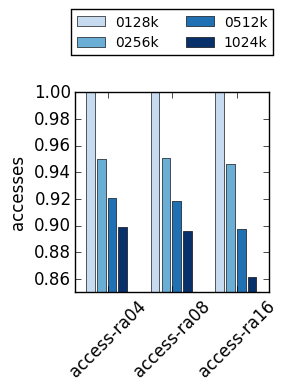
\includegraphics[scale=0.5]{figures/results/speedup/accesses-accesses-0128k-0100-access}
    \caption{Relative number of accesses to L3 cache with varying L2 size.}
    \label{fig:results:l2:access}
\end{figure}

\begin{figure}[!th]
    \centering
    \begin{subfigure}[b]{0.5\textwidth}
        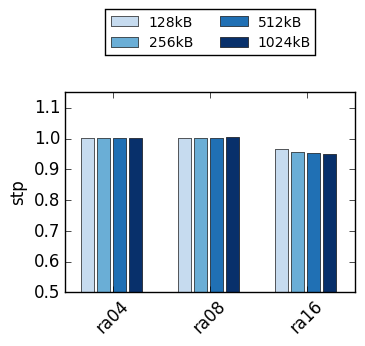
\includegraphics[scale=0.6]{figures/results/speedup/l2-legend-stp-0128k-tadip-l2}
        \caption{Speedup of \gls{tadip} normalized to \gls{lru}.}
        \label{fig:results:l2:tadip}
    \end{subfigure}%
    \begin{subfigure}[b]{0.5\textwidth}
        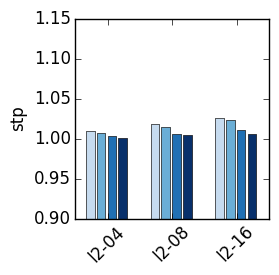
\includegraphics[scale=0.6]{figures/results/speedup/l2-stp-0128k-drrip-3-l2}
        \caption{Speedup of \gls{drrip} normalized to \gls{lru}.}
        \label{fig:results:l2:drrip}
    \end{subfigure}
    \begin{subfigure}[b]{0.5\textwidth}
        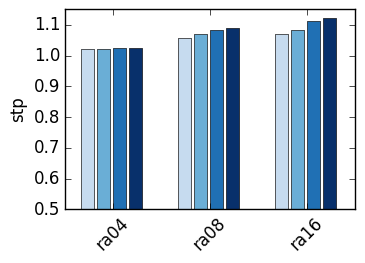
\includegraphics[scale=0.6]{figures/results/speedup/l2-stp-0128k-ucp-l2}
        \caption{Speedup of \gls{ucp} normalized to \gls{lru}.}
        \label{fig:results:l2:ucp}
    \end{subfigure}%
    \begin{subfigure}[b]{0.5\textwidth}
        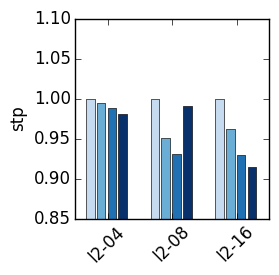
\includegraphics[scale=0.6]{figures/results/speedup/l2-stp-0128k-prism-l2}
        \caption{Speedup of \gls{prism} normalized to \gls{lru}.}
        \label{fig:results:l2:prism}
    \end{subfigure}
    \begin{subfigure}[b]{0.5\textwidth}
        \includegraphics[scale=0.6]{figures/results/speedup/l2-stp-0128k-pipp-l2}
        \caption{Speedup of \gls{pipp} normalized to \gls{lru}.}
        \label{fig:results:l2:pipp}
    \end{subfigure}%
    \begin{subfigure}[b]{0.5\textwidth}
        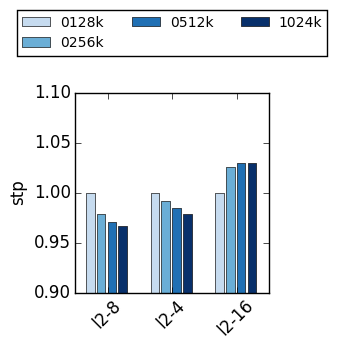
\includegraphics[scale=0.6]{figures/results/speedup/l2-stp-0128k-pipp-min8-l2}
        \caption{Speedup of PIPP-min8 normalized to \gls{lru}.}
        \label{fig:results:l2:pipp-min8}
    \end{subfigure}
    \caption[Speedup with increasing L2 size]{Speedup of cache partition algorithms normalized to \gls{lru} with increasing private L2 size}
    \label{fig:results:l2}
\end{figure}

Figure~\ref{fig:results:l2:tadip} shows the speedup of \gls{tadip} normalized to \gls{lru} measured in \gls{stp}. 
As seen previously, \gls{tadip} performs as good as \gls{lru} in both 4- and 8-core workloads with a 128kB L2 cache.
With increasing L2 cache size \gls{tadip} steadily outperforms \gls{lru} with between 0.1\% and 0.6\% depending on the configuration. 
At 16-cores, \gls{tadip} underperforms compared to \gls{lru}, as previously shown.
We note that, in this case, increasing the L2 size seems to cause a further decrease in \gls{tadip} performance, while the opposite is true in the 8-core case.
We expect that \gls{tadip} will react slower to changes in application phases as memory filtering increases, because of the counter architecture used to switch between algorithms.
This effect does not seem to have a noticeable impact on results for the 4- and 8-core runs, but we assume it is causing the visible decrease in performance for the 16-core runs.

\gls{drrip} as already covered outperforms \gls{lru}, Figure~\ref{fig:results:l2:drrip} confirms this.
The figure also shows that increasing the L2 size causes a reduction in \gls{drrip} performance.
We know that \gls{drrip} uses a step-wise promotion policy where each successive access promotes a block one position.
Naturally less information about successive accesses will be available to the shared level as filtering in the private levels increase.
It is consequently not unexpected that \gls{drrip} suffers from increased filtering by private cache levels.
From the figure, we note that \gls{drrip} seems to be slightly less sensitive to small changes in L2 size with increasing core count, but in all cases a 1024kB L2 causes \gls{drrip} performance to mimic \gls{lru} performance.

In contrast to the previous algorithms, \gls{ucp} performance increases with L2 cache size in all workloads, as seen in Figure~\ref{fig:results:l2:ucp}.
We know that \gls{ucp} uses a utility algorithm as the mechanism for allocating ways to cores. 
The input to this algorithm changes when we increase filtering of requests to the shared cache level.
As a result, the allocation of ways to cores is also expected to change, but this is the intended mechanism of \gls{ucp} and should not negatively affect performance.
\gls{ucp} uses \gls{lru} to manage replacement for each core, but \gls{ucp} under normal circumstances only allows a core to evict one of its own blocks. 
We have already covered that this is why \gls{ucp} outperforms \gls{lru} in the base configuration, in Section~\ref{sec:results:cache_partition}. 
As filtering increases at the private level, we notice that \gls{ucp} increases its performance compared to \gls{lru}. 
We expect that this is because, with increased private cache, more requests from recency-friendly applications can be satisfied by the private levels and less information reaches the shared level.
Trashing and streaming applications will still have its requests propagate to the shared cache, largely independent of the size of the private cache. 
Hence with increasing private cache size we expect \gls{lru} to make worse decisions by prioritizing trashing and streaming patterns due to their access frequency.
\gls{ucp} with utility-based way-partitioning will not suffer as much from the lack of information about recency-friendly applications, and as the results state, can take advantage of increasing private cache size.

\gls{prism} calculates target allocations for each core with the goal of reducing misses.
This technique bears some resemblance to the utility calculation done by the \gls{umon}.
As with \gls{ucp}, we expect \gls{prism} to be able to increase its performance compared to \gls{lru} with increased private cache size because it will continue to limit the cache use of streaming and trashing applications.
We find this expectation reflected in our results.
For both 4- and 16-core workloads we observe an increase in performance compared to \gls{lru} as the size of private cache increases.
In the 8-core results we see the same trend between the smallest and largest L2 configuration, but we unexpectedly observe a performance drop for 256kB and 512kB configurations. 
It is unclear what causes this performance drop, and further work is required to analyze this.

Finally Figure~\ref{fig:results:l2:pipp} show the performance of \gls{pipp}, and Figure~\ref{fig:results:l2:pipp-min8} shows the performance of the modified \gls{pipp} algorithm.
Since \gls{pipp} uses the same utility algorithm as \gls{ucp} and also aims to achieve the same allocations as \gls{ucp}, we expect them to show similar trends.
This expectation somewhat holds true for the 4-core case, where there is a slight upward trend with increasing L2 size.
However, \gls{pipp} underperforms compared to \gls{lru} in all workloads, and with increasing core count performance drops significantly.
We expect the short lifetime of blocks in \gls{pipp} managed caches to be the cause of this, as covered in Section~\ref{sec:results:cache_partition}.
The modified \gls{pipp} algorithm shows a performance development much closer to what is expected, at least for 4- and 8-core workloads.
We observe the same increase in performance with increased L2 cache size as seen in the \gls{ucp} case. 
In the 16-core workloads, the performance trend is still as expected, but the modified algorithm performs worse than \gls{lru}.
This performance reduction for larger core counts has also been observed in previous research~\cite{Manikantan2012}.
